\documentclass[a2paper, 12pt]{article}
\usepackage[font={huge, bf}]{caption}
\usepackage{fontspec}
\setmainfont{Arial}
\usepackage{subcaption}
\usepackage{graphicx}
\usepackage{tikz}
\usepackage{tikzsymbols}
\usetikzlibrary{calc,patterns,shapes.geometric}
\usepackage{float}
\usepackage{pdflscape}
\usepackage{geometry}
\geometry{landscape, margin=2cm}
\captionsetup[subfigure]{justification=justified,singlelinecheck=false}
\pagestyle{empty}

\def\centerarc[#1](#2)(#3:#4:#5){\draw[#1] ($(#2)+({#5*cos(#3)},{#5*sin(#3)})$) arc (#3:#4:#5);}

\begin{document}
	\vspace*{\fill}
	\begin{figure}[!htbp]
		\centering
		\begin{subfigure}[b]{0.48\textwidth}
			\caption{Figure 1}
			\centering
			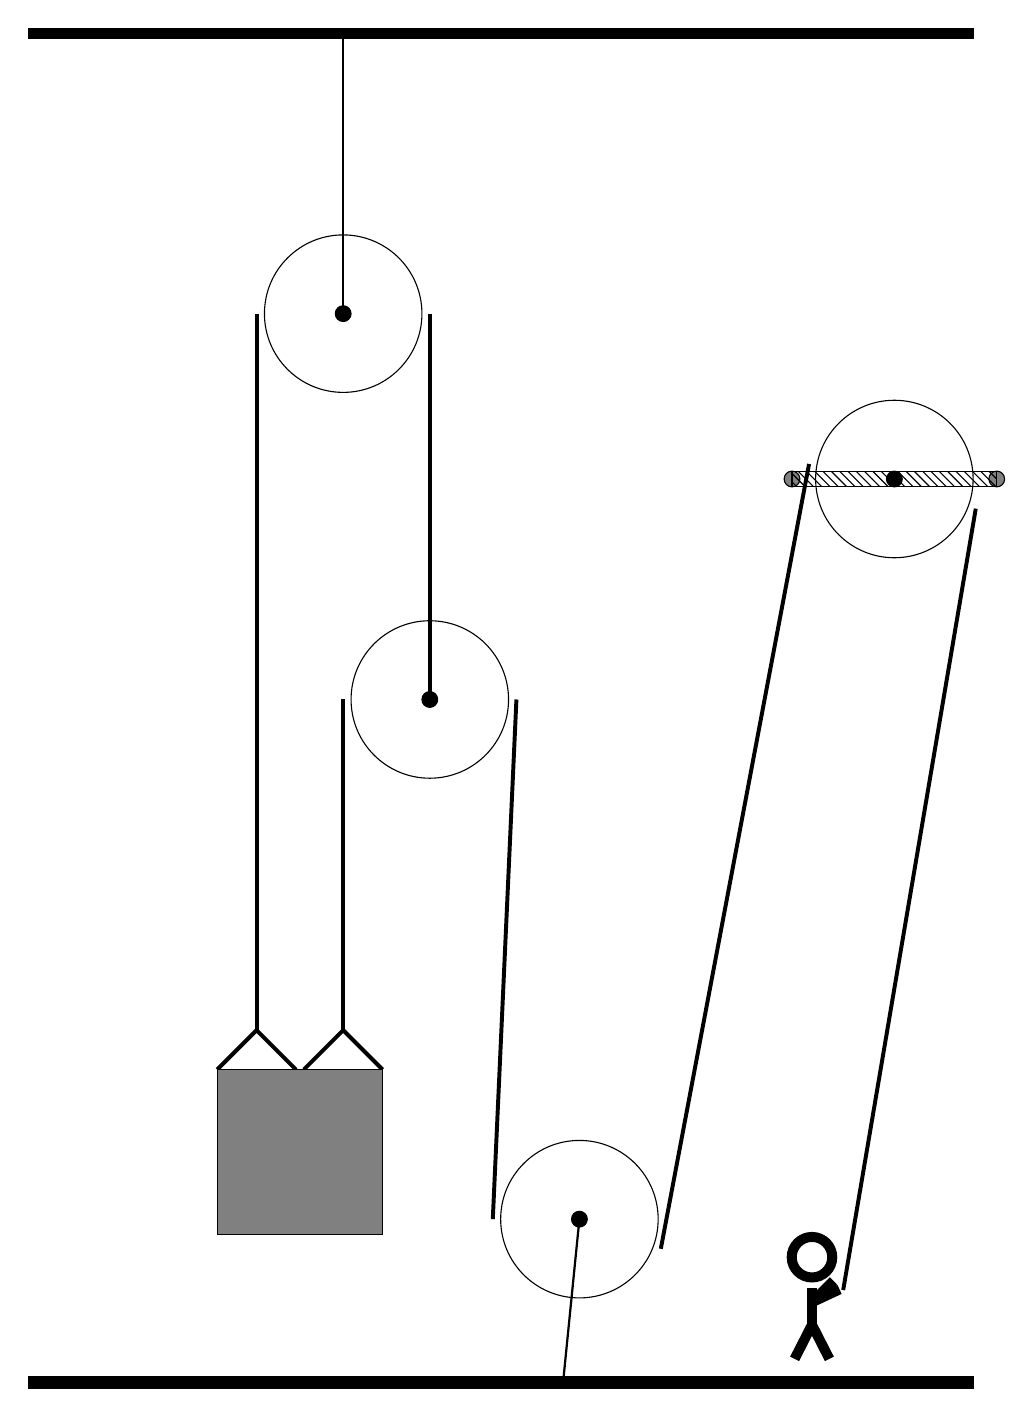
\begin{tikzpicture}
				\draw[fill=black] (-2, 14) rectangle (10, 14.125);
				
				\draw (2, 10.5) circle (1);
				\draw[fill=black] (2, 10.5) circle (0.1);
				\draw[thick] (2, 10.5) -- (2, 14);
				
				\draw (3.1, 5.6) circle (1);
				\draw[fill=black] (3.1, 5.6) circle (0.1);
				
				\draw (5, -1) circle (1);
				\draw[fill=black] (5, -1) circle (0.1);
				\draw[thick] (5, -1) -- (4.8, -3);
				
				\draw (9, 8.4) circle (1);
				\draw[fill=black] (9, 8.4) circle (0.1);
				\draw[fill=black!50] (7.7, 8.4) circle (0.1);
				\draw[fill=black!50] (10.3, 8.4) circle (0.1);
				\draw[pattern=north west lines, pattern color=black] (7.7, 8.5) rectangle (10.3, 8.3);
				
				\draw[line width = 0.5mm]  (0.4, 0.9) -- (0.9, 1.4) -- (1.4, 0.9);
				\draw[line width = 0.5mm]  (1.5, 0.9) -- (2.0, 1.4) -- (2.5, 0.9);
				\draw[fill=black!50] (0.4, 0.9) rectangle (2.5, -1.2);
				
				\draw[line width = 0.5mm] (0.9, 10.5) -- (0.9, 1.4);
				\centerarc[line width = 0.5mm](2, 10.5)(0:180:1.1);
				\draw[line width = 0.5mm] (3.1, 10.5) -- (3.1, 5.6);
				\draw[line width = 0.5mm] (2.0, 5.6) -- (2.0, 1.4);
				\centerarc[line width = 0.5mm](3.1, 5.6)(0:180:1.1);
				\draw[line width = 0.5mm] (4.2, 5.6) -- (3.9, -1);
				\centerarc[line width = 0.5mm](5, -1)(180:340:1.1);
				\draw[line width=0.5mm](6.0337, -1.3762) -- (7.9167, 8.591);
				\centerarc[line width = 0.5mm](9, 8.4)(-20:170:1.1);
				\draw[line width=0.5mm](10.0337, 8.0238) --  (8.35, -1.9);
				
				\node at (8, -2) {\scriptsize \Strichmaxerl[10][225][25]};
				
				\draw[fill=black] (-2, -3) rectangle (10, -3.15);
			\end{tikzpicture}
		\end{subfigure}
		\hfill
		\begin{subfigure}[b]{0.48\textwidth}
			\caption{Figure 2}
			\centering
			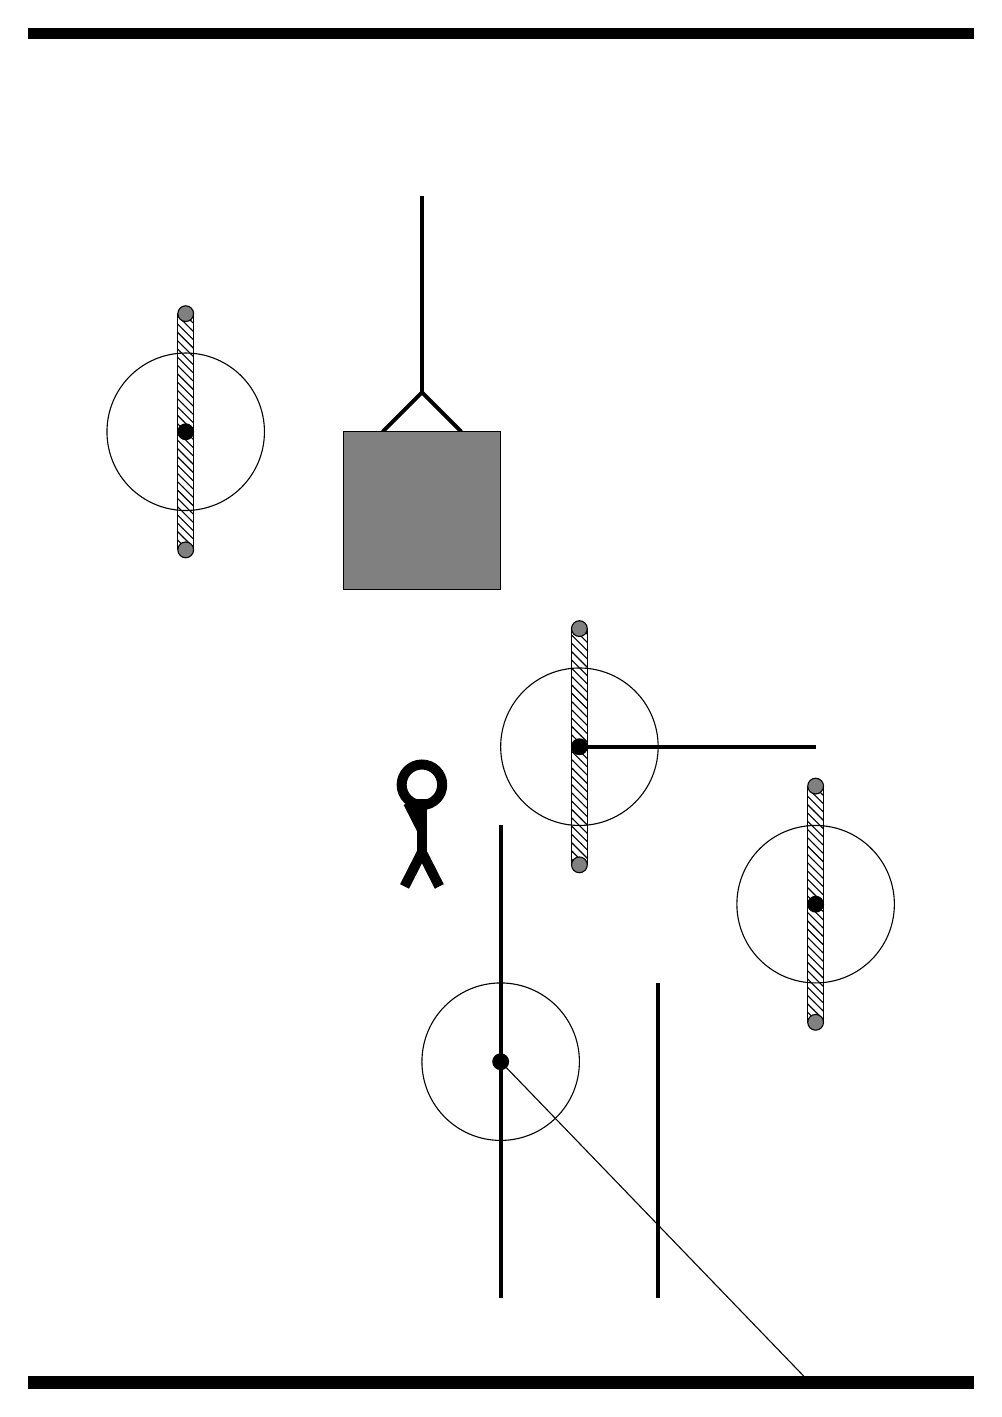
\begin{tikzpicture}
				\draw[fill=black] (-2, 14) rectangle (10, 14.125);
				
				\draw (0,9) circle (1);
				\draw[fill=black] (0,9) circle (0.1);
				\draw[pattern=north west lines, pattern color=black] (-0.1,10.5) rectangle (0.1,7.5);
				\draw[fill=black!50] (0,10.5) circle (0.1);
				\draw[fill=black!50] (0,7.5) circle (0.1);
				
				\draw (4,1) circle (1);
				\draw[fill=black] (4,1) circle (0.1);
				\draw (8,-3.15) -- (4,1);
				
				\draw (8,3) circle (1);
				\draw[fill=black] (8,3) circle (0.1);
				\draw[pattern=north west lines, pattern color=black] (7.9,4.5) rectangle (8.1,1.5);
				\draw[fill=black!50] (8,4.5) circle (0.1);
				\draw[fill=black!50] (8,1.5) circle (0.1);
				
				\draw (5,5) circle (1);
				\draw[fill=black] (5,5) circle (0.1);
				\draw[pattern=north west lines, pattern color=black] (4.9,6.5) rectangle (5.1,3.5);
				\draw[fill=black!50] (5,6.5) circle (0.1);
				\draw[fill=black!50] (5,3.5) circle (0.1);
				
				\draw[line width=0.5mm](3,9.5) -- (3,12.0);
				\draw[line width=0.5mm](2.5,9) --  (3,9.5) -- (3.5,9);
				\draw[fill=black!50] (2, 9) rectangle (4, 7);
				
				\draw[line width = 0.5mm] (5,5) -- (8,5);
				\centerarc[line width = 0.5mm](5,4)(90:180:1);
				\draw[line width = 0.5mm] (4,4) -- (4,-2);
				\centerarc[line width = 0.5mm](5,-2)(180:360:1);
				\draw[line width = 0.5mm] (6,-2) -- (6,2);
				
				\node at (3, 4) {\scriptsize \Strichmaxerl[10][-63][90]};
				
				\draw[fill=black] (-2, -3) rectangle (10, -3.15);
			\end{tikzpicture}
		\end{subfigure}
	\end{figure}
		\vspace*{\fill}
\end{document}